%----------------------------------------------------------------------------
% Start
%----------------------------------------------------------------------------

\documentclass{article}

\usepackage{graphicx} % Required for the inclusion of images
\usepackage{tocloft}
\usepackage[nottoc,numbib]{tocbibind} % Reference in TOC and numbered
\usepackage{url} % Reference include URL

\renewcommand{\cftsecleader}{\cftdotfill{\cftdotsep}}
\renewcommand{\labelenumi}{\alph{enumi}.}

\setlength\parindent{0pt} % Removes all indentation from paragraphs


%----------------------------------------------------------------------------
% Document Information
%----------------------------------------------------------------------------

\begin{titlepage}

\title{Giguesaur: Game Logic}
\author{Ashley Manson}
\date{\today}

\begin{document}
\maketitle

\begin{center}
Co-Workers: Joshua La Pine \& Shahne Rodgers\\
Supervisors: Geoff Wyvill \& David Eyers\\

\vspace*{1\baselineskip} % Skip a line

Dept. of Computer Science\\
University of Otago
\end{center}

\end{titlepage}

%----------------------------------------------------------------------------
% Table of Contents
%----------------------------------------------------------------------------

\tableofcontents
\newpage

%----------------------------------------------------------------------------
% Introduction
%----------------------------------------------------------------------------

\section{Introduction}

Our vision for our completed Giguesaur application was allowing a classroom of children, each with their their own iPad, to run around and solve a jigsaw puzzle together. Imagine a classroom full of kids where they are all trying to work on a single conventional jigsaw puzzle; such a scheme is in no way pratical. The main goal of our project, besides all the design and technical subgoals, is simply to make a that is fun for children to play and work together.

% Overview of the project
\subsection{Overview}
The Giguesaur application development was divided into three different components. Joshua La Pine was in charge of developing the computer vsion part of the project, which allows for the puzzle pieces to be rendered over top the 'game board' in the real world. Shahne Rodgers took charge of the networking component of the project, which was crucial in allowing more than one player to interact with the jigsaw puzzle. Finally my part of the project was to develop the game logic and render the game to the iPad's screen.

% Background including what a puzzle is and other games
\subsection{Background}
There are many jigsaw puzzle games that are available for iOS and other hand-held devices, such as Magic Jigsaw Puzzles \cite{ref:MagicJigsaw} and Jigsaw Puzzle \cite{ref:JigsawPuzzle}, but the majority of them are limited in the way they look due to them using an orthographic projection to render the jigsaw puzzles. What this projection means is that the puzzle pieces of the jigsaw puzzle are flat on the screen, the player can only look at the jigsaw puzzle from top down, there is no depth and all the puzzle pieces are displayed as the same size. This is something that does not work for the Giguesaur project as the puzzle pieces are rendered in a perspective projection, so when the jigsaw puzzle is rendered onto the game board it looks more realistic, as puzzle pieces that are further away from the camera are shown to be smaller than pieces that are closer to the camera. Another limitation of jigsaw puzzle games is the way they can be interacted with, by which I mean the way they can be solved. The puzzle pieces have to be placed into a predefined grid. Farms And Animals Puzzles \cite{ref:FarmPuzzle} is an example of a game that has this grid layout for the puzzle pieces to be placed in, which is shown in figure \ref{fig:FarmsAnimals}, it also shows the limited orthographic perspective of the game. This means that all the puzzle pieces will be placed in the centre of the screen. This is something that was illogical for the project and I did not want to limit the scope of the game. I have made it possible for the jigsaw puzzle to be solved anywhere on the board, be it in the centre of the game board or off in a corner of the game board. I also believe that it makes for a more interesting game.

\begin{figure}[h]
\begin{center}
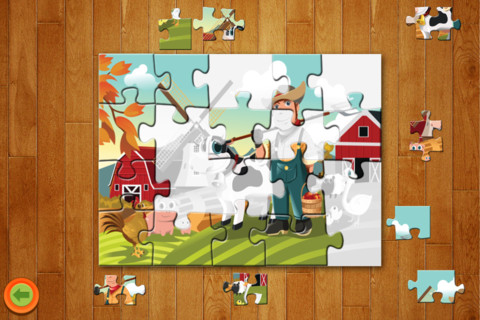
\includegraphics[width=0.85\textwidth]{images/FarmAnimalsJigsawImage}
\caption{Screenshot of Farms And Animals Puzzles \cite{img:FarmPuzzle}.}
\label{fig:FarmsAnimals}
\end{center}
\end{figure}

\subsection{iOS}


% Brief introduction on my work
\subsection{Game Logic}
As I stated previously, I was in charge of developing the game logic for the Giguesaur game.

%---------------------------------------------------------------------------
% Work Done
%---------------------------------------------------------------------------

\section{Work Done}

% Work done on Mac
\subsection{Start of Development}

% This is the build that had perspective stuff
\subsection{Prototype}

% Porting to iPad including changes and problems incountered
\subsection{Port to iPad}

% Integrating with others including problems incountered
\subsection{Integration}

%---------------------------------------------------------------------------
% Results
%---------------------------------------------------------------------------

\section{Results}

%---------------------------------------------------------------------------
% Conclusion
%---------------------------------------------------------------------------

\section{Conclusion}

% What the thing looks like
\subsection{Final Build}

% What hasn't been done
\subsection{Future Work}

\subsection{Final Words}

%---------------------------------------------------------------------------
% References
%---------------------------------------------------------------------------

\clearpage
\bibliographystyle{ieeetr}
\bibliography{references}

%---------------------------------------------------------------------------
% End
%---------------------------------------------------------------------------

\end{document}
